\begin{figure}[H]
	\centering
	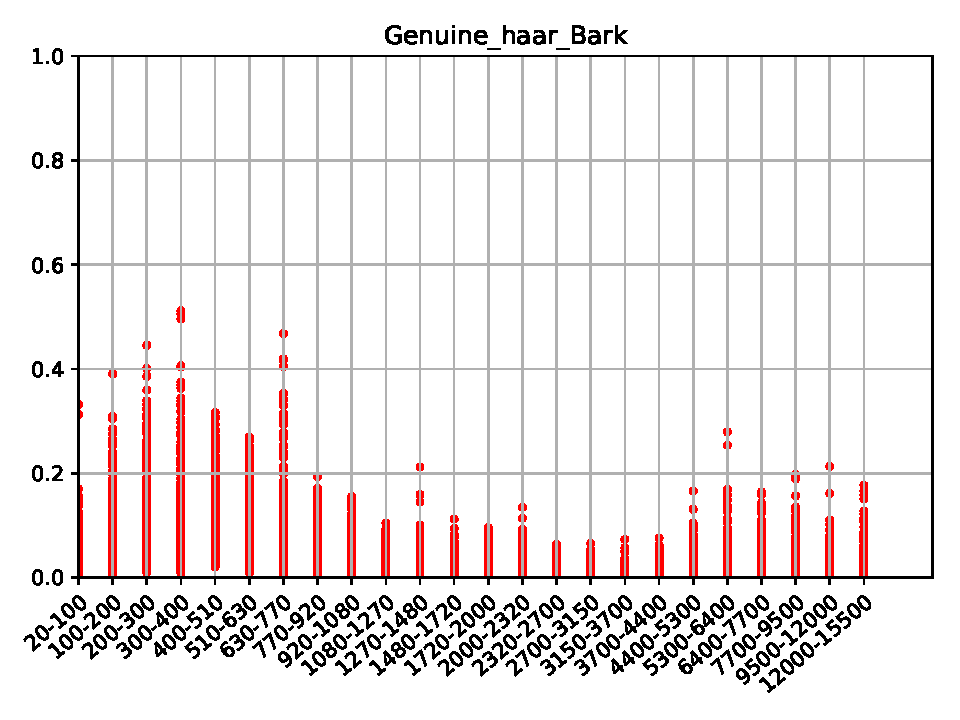
\includegraphics[scale=.8]{./images/results/barkVersusMel/Genuine_haar_Bark.pdf}
	\caption{Gráfico de dispersão para os vetores de características \textit{genuínos} obtidos com \textit{Haar + BARK}. Eixos horizontais e verticais: Bandas de frequência em Hertz(Hz) e amplitudes, respectivamente.}
	\label{fig:livehaarbark}
\end{figure}
\begin{figure}[H]
	\centering
	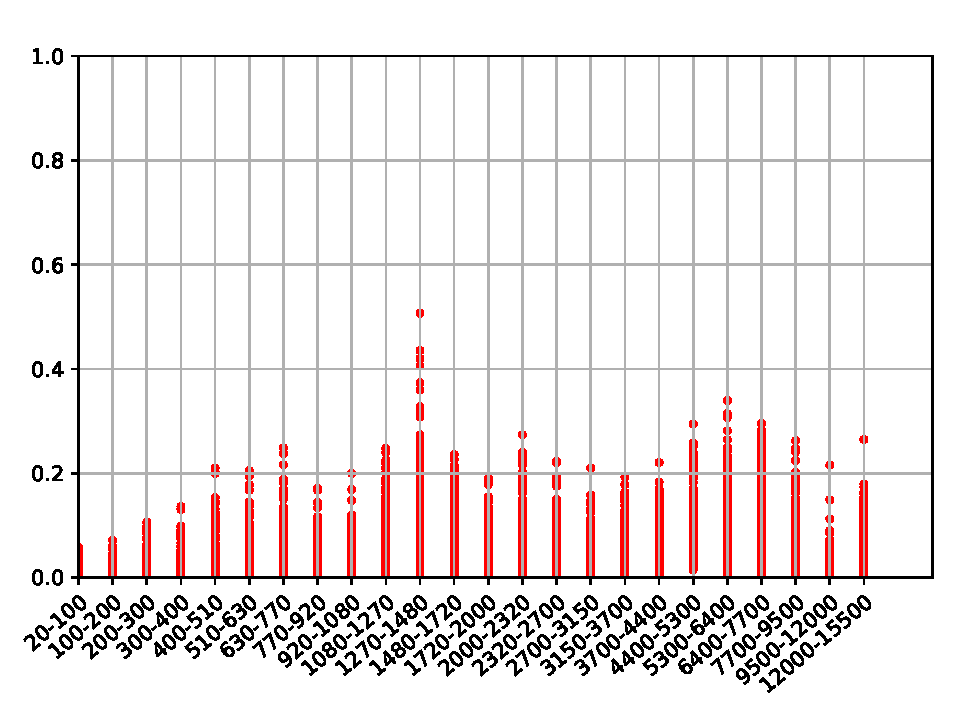
\includegraphics[scale=.8]{./images/results/barkVersusMel/Spoofing_haar_Bark.pdf}
	\caption{Gráfico de dispersão para os vetores de características \textit{falseados} obtidos com \textit{Haar + BARK}. Eixos horizontais e verticais: Banda de frequência em Hertz(Hz) e amplitudes, respectivamente.}
	\label{fig:spoofinghaarbark}
\end{figure}
\begin{figure}[H]
	\centering
	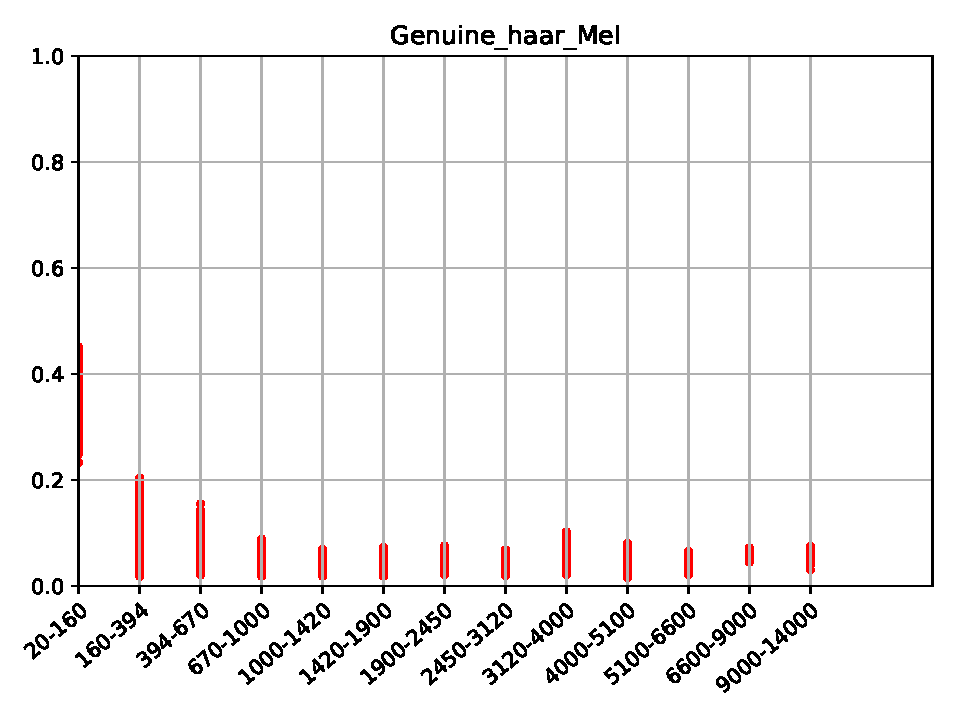
\includegraphics[scale=.8]{./images/results/barkVersusMel/Genuine_haar_Mel.pdf}
	\caption{Gráfico de dispersão para vetores de características \textit{genuínos} obtidos com \textit{Haar + MEL}. Eixos horizontais e verticais: Bandas de frequência em Hertz(Hz) e amplitudes, respectivamente.}
	\label{fig:livehaarmel}
\end{figure}
\begin{figure}[H]
	\centering
	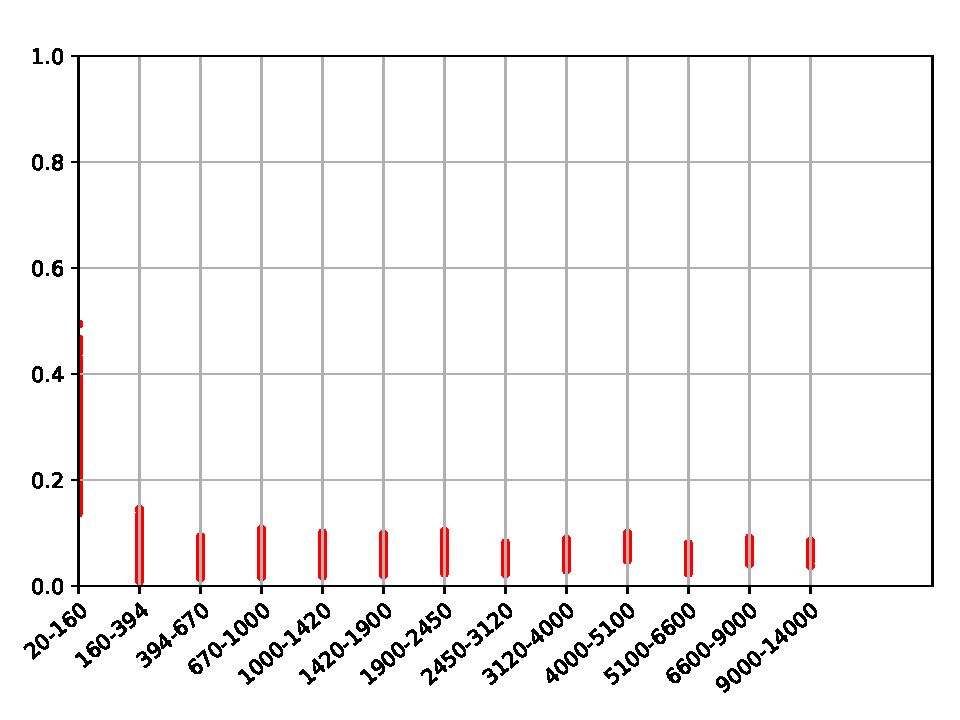
\includegraphics[scale=.8]{./images/results/barkVersusMel/Spoofing_haar_Mel.pdf}
	\caption{Gráfico de dispersão para vetores de características \textit{falseados} obtidos com \textit{Haar + MEL}. Eixos horizontais e verticais: Bandas de frequência em Hertz(Hz) e amplitudes, respectivamente.}
	\label{fig:spoofinghaarmel}
\end{figure}
\begin{figure}[H]
	\centering
	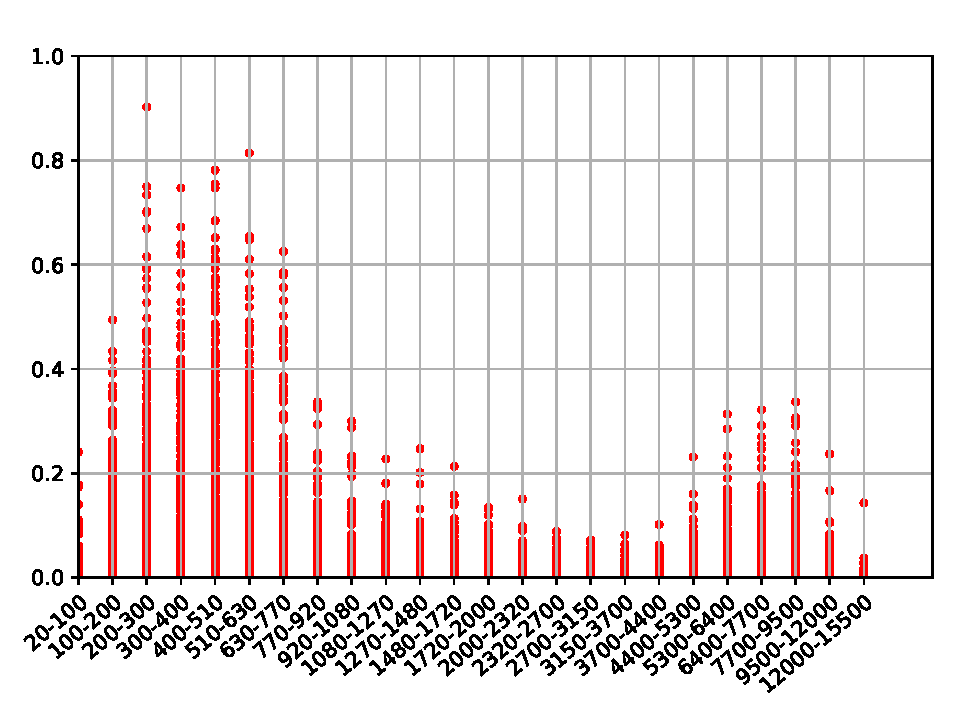
\includegraphics[scale=.8]{./images/results/barkVersusMel/Genuine_daub76_Bark.pdf}
	\caption{Gráfico de dispersão para vetores de características \textit{genuínos} obtidos com \textit{daubechies 76 + BARK}.  Eixos horizontais e verticais: Bandas de frequência em Hertz(Hz) e amplitudes, respectivamente.}
	\label{fig:livedaub76bark}
\end{figure}
\begin{figure}[H]
	\centering
	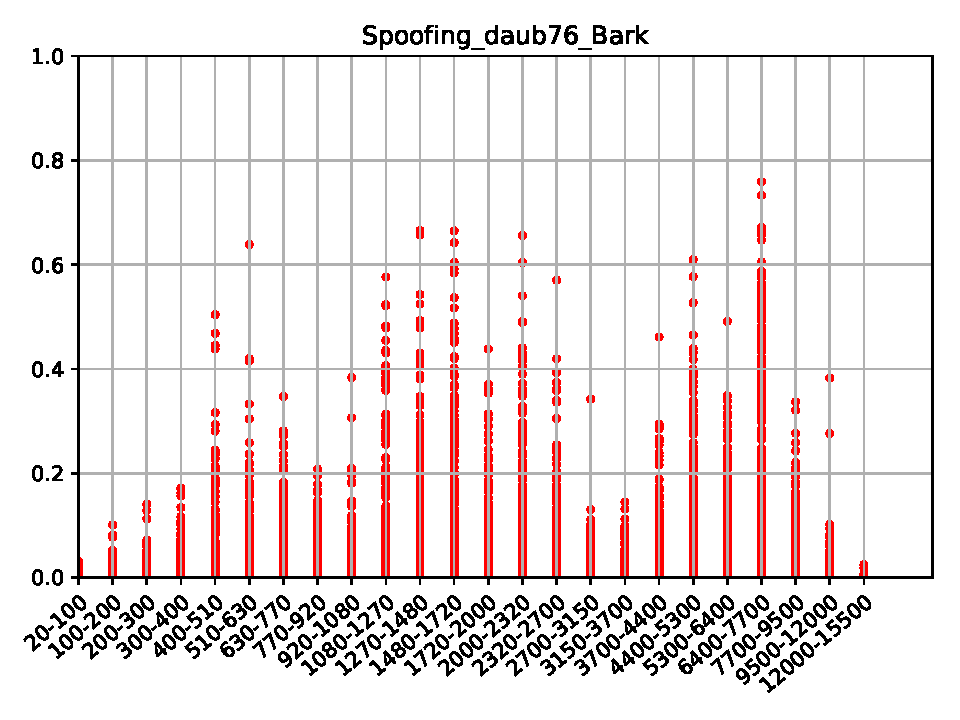
\includegraphics[scale=.8]{./images/results/barkVersusMel/Spoofing_daub76_Bark.pdf}
	\caption{Gráfico de dispersão para vetores de características \textit{falseados} obtidos com \textit{daubechies 76 + BARK}.  Eixos horizontais e verticais: Bandas de frequência em Hertz(Hz) e amplitudes, respectivamente.}
	\label{fig:spoofingdaub76bark}
\end{figure}
\begin{figure}[H]
	\centering
	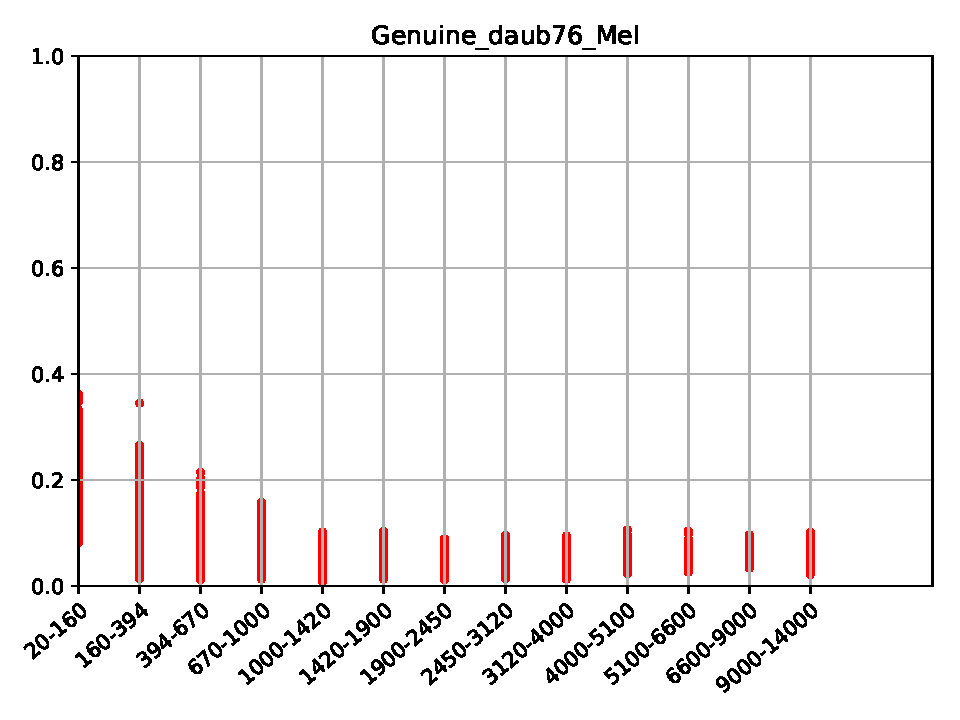
\includegraphics[scale=.8]{./images/results/barkVersusMel/Genuine_daub76_Mel.pdf}
	\caption{Gráfico de dispersão para vetores de características \textit{genuínos} obtidos com \textit{daubechies 76 + MEL}.  Eixos horizontais e verticais: Bandas de frequência em Hertz(Hz) e amplitudes, respectivamente.}
	\label{fig:livedaub76mel}
\end{figure}
\begin{figure}[H]
	\centering
	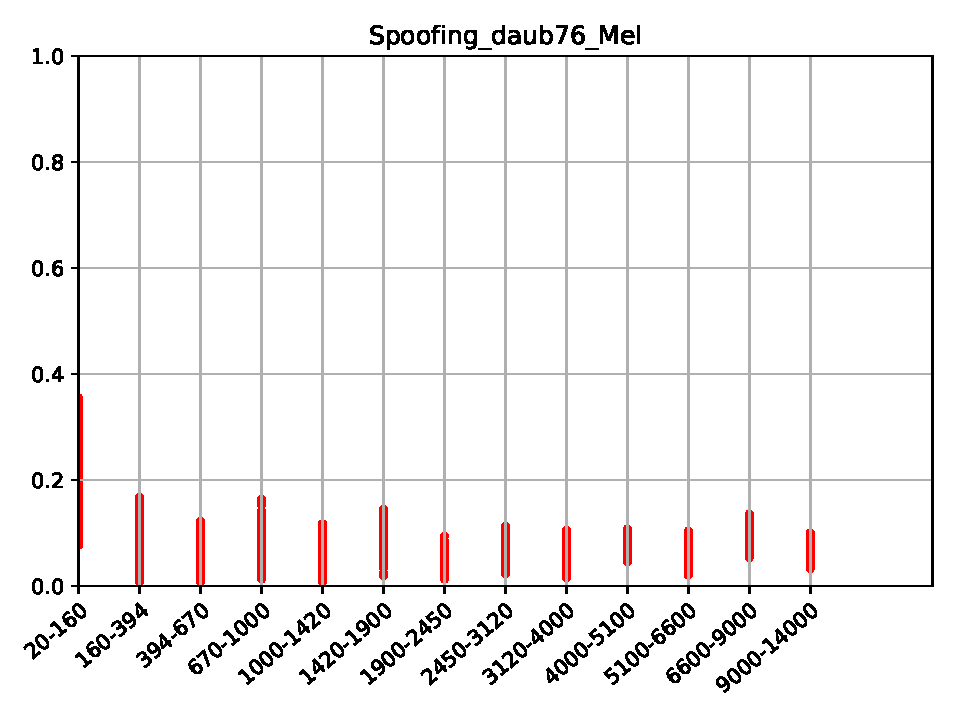
\includegraphics[scale=.8]{./images/results/barkVersusMel/Spoofing_daub76_Mel.pdf}
	\caption{Gráfico de dispersão para vetores de características \textit{falseados} obtidos com \textit{daubechies 76 + MEL}.  Eixos horizontais e verticais: Bandas de frequência em Hertz(Hz) e amplitudes, respectivamente.}
	\label{fig:spoofingdaub76mel}
\end{figure}